\newpage
\part{Biokemiske processer}
    \part{Forklar de 2 biokemiske processer respiration og fotosyntese.}
        \subsection*{Respiration}\label{sec:respiration}
            I en eukaryot celle sker respirationen i mitokondrierne. Respiration er en proces, hvor celler nedbryder glucose til at frigive energi, i from af ATP.
            Den formel som beskriver respirationen er: \begin{equation}C_6H_{12}O_6 + 6CO_2 \rightarrow 6O_2 + 6H_2O + ATP \end{equation}+
            Respiration kan deles op i 3 dele, hhv. glykolysen, citronsyrecyklus og elektrontransportkæden.

            \subsubsection*{Glykolysen}
                Glykolyse er den første fase af cellulær respiration, den proces, hvor celler genererer energi fra næringsstoffer. Glykolyse sker i cytoplasmaet i cellen og er en anaerob proces, hvilket betyder, at den ikke kræver ilt. Under glykolyse omdannes en molekyle glucose til to molekyler af en forbindelse kaldet pyruvat (\begin{math}C_3H_4O_3\end{math}). I glukolysen produceres der også 2 ATP-molekyler. Dette er en af to måder der kan dannes ATP på under respiration. Den form for ATP produktion kaldes for substrat fosforylering. glukolysen er den eneste del af respirationen som kan foregå uden ilt. Hvis der ikke er Ilt kan pyruvat ikke indgå  i respirationens næste trin. I stedet vil pyruvaten blive brugt til fermentering og det vil derfor blive lavet om til Laktat eller Ethanol, dette er en anaerob process som ikke kræver ilt og derfor kan foregå uden ilt. Men hvis nu der er ilt kan det gå videre til næste trin i respirationen. Pyruvatet skal altså nu transporterers ind i mitokondrierne. Når pyovaten efter glukolysen bliver transporteret ind i mitokondrierne vil der blive fraspaltet \begin{math}
                CO_2\end{math} Før næste fase kan gå igang. 

            \subsubsection*{Citronsyrecyklus}
                Den pyruvat der bliver tilført er en carbon forbindelse, de carbon atomer kommer ud som \begin{math}CO_2\end{math}. Der dannes også ATP i denne fase på samme måde som for oven.

            \subsubsection*{Elektrontransportkæden}
                \begin{figure}
                    \centering
                    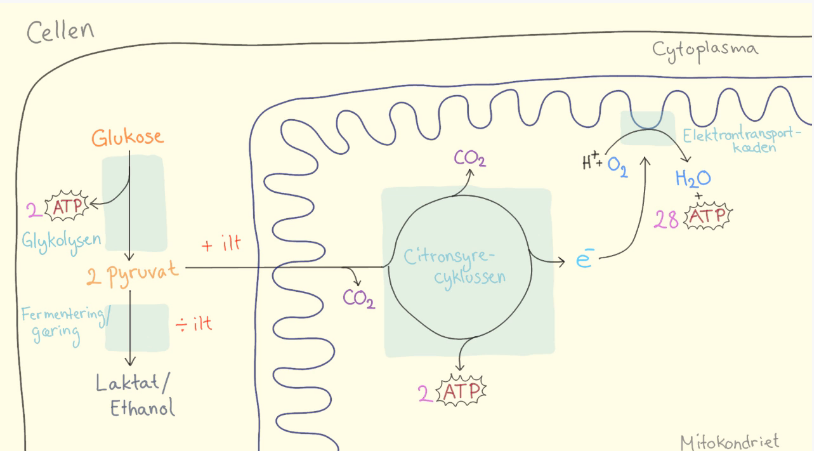
\includegraphics[width=0.5\textwidth]{figurs/respiration.png}
                    \caption{Respiration}
                    \label{fig:respiration}
                \end{figure}
                \newpage
                
        \subsection*{Fotosyntese}
            I en eukaryot plantecelle har man et organell som man ikke har i en eukaryot dyre celle, nemlig grønkorn. I grønkornene sker der en masse biokemiske processer som vi tilsammen kalder for fotosyntese. Under fotosyntese dannes to vigigtige stoffer, nemlig glucose og ilt. glucose (\begin{math}C_6H_{12}O_6\end{math}) er en sukkerart som er vigtig for planten, da den bruger den til at danne andre stoffer som den har brug for. 
            \begin{math}O_2\end{math} er ilt, som er vigtigt for alle levende organismer, da det er det vi bruger til at danne energi her i blandt \ref{sec:respiration}.
            I fotosyntese skal planten bruge to ting \begin{math}CO_2\end{math} og \begin{math}H_2O\end{math}. Alt det førnævte er ting som planten optager fra det miljø den er i. De to stoffer bruges til at skabe det organiske stof glucose. Glucose er et meget energirigt stof derfor kræve fotosyntese lysenergi. Heraf foto-syntese (lys drevet syntese)  \begin{math}H_2O\end{math} er vand, som planten optager fra jorden.
            Den simple formel for fotosyntese er: \begin{equation} 6CO_2 + 6H_2O \rightarrow C_6H_{12}O_6 + 6O_2 \end{equation}\label{eq:fotosyntese}
            Fotosyntese består af de 15-20 delprocesser, som overall kan beskrives med den fromel som ses ovenfor. (Se afsnit \ref{eq:fotosyntese})
            Man kan dele disse processer op i to dele hhv mørke- og lysprocessen. \newline 
            \subsubsection*{Lysprocessen}
                Lys processerne kræver lys og kan kun foregå når der er lys til stede. Lysprocessen sker i thylakoiderne. I processen bliver der brugt \begin{math}H_2O\end{math} O som bliver lavet om til ilt og hydrogen. Hydrogen bliver hoverført til \begin{math}NADP^+\end{math} så det danner \begin{math}NADPH\end{math} (\begin{math}NADPH\end{math} er et organiske molekyle.) 
                Lysenergien anvendes til at sammensætte \begin{math}ADP + P_i\end{math} Og på den måde omdannes \begin{math}ADP\end{math} og \begin{math}P_i\end{math} til \begin{math}ATP\end{math} Denne process er afhængig af chloroflyl (Det som absorbere lysenergien) under lysprocessen dannes altså \begin{math}ATP\end{math} og \begin{math}NADPH\end{math} og ilt. En del af ilten bruges til respiration (se afsnit \ref{sec:respiration}), mens resten af ilten frigives til atmosfæren. Hele mængden af \begin{math}ATP\end{math} og \begin{math}NADPH\end{math} bruges i mørkeprocessen. 

            \subsubsection*{Mørkeprocessen}
                Mørkeprocessen er den del af fotosyntesen som ikke kræver lys. Denne proces foregår i grønkornene, dog uden for thylakoidmembranerne. Denne proces er en meget kompleks proces. 
                Under mørkeprocessen optager planten Kuldioxid, under forbrug af kemisk energi fra ATP kombineres \begin{math}CO_2\end{math} med hydrogen fra \begin{math}NADPH\end{math} til at danne glukose(\begin{math}C_6H_{12}O_6\end{math}). Mørkeprocessen er ikke direkte afhængig af lys. Men den er helt afhængig af produkterne der kommer fra lysprocessen (\begin{math}ATP\end{math} og \begin{math}NADPH\end{math}). Selv om man kalder det for mørkeprocessen sker processen især når planten modtager lys, derfor ville man kunne give den et mere passende navn det kunne være "De enzymatiske processer"
            \subsubsection*{Opsumering} 
                Under den samlede fotosyntese fungere NADPH altså som hydrogen transportør fra lys- til mørkeprocesser. Mens ATP fungere som energi transportør fra lys- til mørkeprocesser. Lige som i respiration dannes ATP under fotosyntese. Ved respiration forlader ATP mitokondrierne og bruges andre steder i cellen. Ved fotosyntese forlader ATP aldrig grønkornene men bruges til fulde i mørkeprocessen.
                \begin{figure}[h]
                    \centering
                    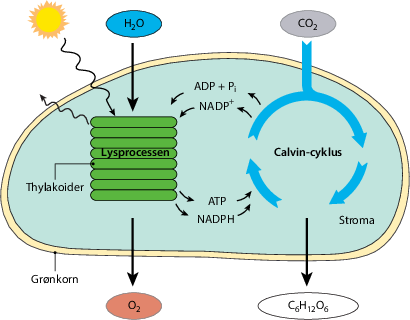
\includegraphics[width=0.8\textwidth]{figurs/fotosyntese.png}
                    \caption{Fotosyntese}
                    \label{fig:fotosyntese}
                \end{figure}

    \newpage
    \section*{Redegør for øvelsen: Fotosyntese og Respiration hos vandpest.}
        \begin{figure}
            \centering
            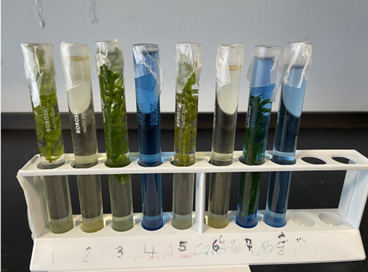
\includegraphics[width=0.8\textwidth]{figurs/forsogVandpeast.png}
            \caption{Fotosyntese og Respiration hos vandpest}
            \label{fig:versus}
        \end{figure}
    \section*{Diskuter hvordan de 2 processer kan have indflydelse på klimaet.}
        Fotosyntese og cellulær respiration er to fundamentale biologiske processer, der har betydelig indflydelse på klodens klima. 
        Disse to processer er tæt forbundet i det, der ofte kaldes den globale kulstofcyklus. Fotosyntese trækker CO2 ud af atmosfærn, mens cellulær respiration og andre biologiske og geologiske processer frigiver CO2 tilbage i atmosfæren og oceanerne.
        Hvis disse processer er i balance, forbliver mængden af CO2 i atmosfæren stort set konstant. Men menneskelige aktiviteter, såsom brænding af fossile brændstoffer og skovrydning, har forstyrret denne balance ved at øge mængden af CO2, der frigives til atmosfæren, og ved at reducere antallet af planter, der kan fjerne CO2 gennem fotosyntese. Dette har bidraget til en stigning i atmosfærens CO2-indhold og global opvarmning.
        Desuden spiller fotosyntese og respiration også en rolle i vandcyklussen, som har indflydelse på klimamønstre og vejrsystemer. For eksempel frigives vanddamp til atmosfæren under transpiration (en del af fotosyntesen), hvilket bidrager til skydannelse og nedbør. På den anden side producerer respiration også vand, der kan blive genbrugt i forskellige biologiske processer.
        Samlet set er fotosyntese og cellulær respiration centrale for livet på Jorden og spiller en vigtig rolle i reguleringen af klodens klima.